\begin{artengenv}{Krzysztof Sołoducha}
	{Analysis of the implications of the Moral Machine project as an implementation of the concept of coherent extrapolated volition for building clustered trust in autonomous machines}
	{Analysis of the implications of the Moral Machine project\ldots}
	{Analysis of the implications of the Moral Machine project as\\an implementation of the concept of coherent extrapolated volition\\for building clustered trust in autonomous machines}
	{Military University of Technology}
	{In this paper, we focus on the analysis of Eliezer Yudkowsky's concept of ``coherent extrapolated volition'' (CEV) as a~response to the need for a~post-conventional, persuasive morality that meets the criteria of active trust in the sense of Anthony Giddens, which could be used in the case of autonomous machines. Based on the analysis of the results of the Moral Machine project, we formulate some guidelines for transformation of the idea of a~coherent extrapolated volition into the concept of a~coherent, extrapolated and clustered volition. The argumentation used in the paper is intended to show that the idea of CEV transformed into its clustered version can be used to build a~technically and socially efficient decision-making pattern database for autonomous machines.
	}
	{ethics of artificial intelligence, ethics of autonomous machines, trust in artificial intelligence, moral machine project, coherent extrapolated volition.}
	
	
%\begin{document}
%\title{Analysis of the implications of the ``Moral Machine'' project as an implementation of the concept of ``coherent, extrapolated volition'' for building clustered trust in autonomous machines}
%\maketitle
%
%Krzysztof Sołoducha PhD, prof. WAT \href{mailto:krzysztof.soloducha@wat.edu.pl}{krzysztof.soloducha@wat.edu.pl}
%
%\section{Abstract}
%\begin{quotation}
%In this paper, we focus on the analysis of Eliezer Yudkowsky's concept of ``coherent extrapolated volition'' (CEV) as a~response to the need for a~post-conventional, persuasive morality that meets the criteria of active trust in the sense of Anthony Giddens, which could be used in the case of autonomous machines. Based on the analysis of the results of the Moral Machine project, we formulate some guidelines for transformation of the idea of a~coherent extrapolated volition into the concept of a~coherent, extrapolated and clustered volition. The argumentation used in the paper is intended to show that the idea of CEV transformed into its clustered version can be used to build a~technically and socially efficient decision-making pattern database for autonomous machines.
%
%\end{quotation}
%\section{Key words}
%\begin{quotation}
%ethics of artificial intelligence, ethics of autonomous machines, trust in artificial intelligence, moral machine project, coherent extrapolated volition
%
%\end{quotation}



\lettrine[loversize=0.13,lines=2,lraise=-0.03,nindent=0em,findent=0.2pt]%
{T}{}he problem of the ethics of autonomous machines is a~philosophical issue that has emerged together with the dangers of the development of modern technologies that allow the autonomisation of machine operation
%\label{ref:RNDCNwvoNhD5U}(Pasquale, 2016).
\parencite[][]{pasquale_black_2016}. %
 Of course, the classic of considerations on this issue is Isaac Asimov 
%\label{ref:RND8EDGzYgvVE}(2004)
\parencite*[][]{asimov_runaround_2004} %
 and his reflections on the ethics of robots, but at the moment the discussion on this topic is determined primarily by the dynamic development of unsupervised machine learning methods 
%\label{ref:RNDZsSSj9nxYT}(Gryz, 2021).
\parencite[][]{gryz_sztuczna_2021}. %
 They have gained a~second wind (having been theoretically developed in the 1980s) thanks to the development of the Internet and access to large sets of data on which machines can learn and improve algorithms on their own, using formal rules of statistical reasoning and without any kind of supervision 
%\label{ref:RND2WtqnrZTv3}(Burrell, 2016).
\parencite[][]{burrell_how_2016}.%


This development brings certain risks. The most popular technologies based on the statistical paradigm, i.e. deep neural networks (more than 5 layers) or multilevel neural networks (such as Deepmind's AlphaGo), tend to have problems with a~lack of transparency and explainability, which are currently the subject of intense discussion in the community related to the philosophy of artificial intelligence
%\label{ref:RNDkgdYGGullO}(Eschenbach, 2021).
\parencite[][]{eschenbach_transparency_2021}. %
 There are considerations concerning so called black box problem 
%\label{ref:RNDnydtOYQIDO}(Pasquale, 2016).
\parencite[][]{pasquale_black_2016}.%


The classic problem of the ethics of robot activity raised by Asimov has thus been transformed today into a~consideration of the concept of \textit{benevolence}—the result of which is to build machines that do Good, especially under the threat of singularity. It means that machines are expected to act in favour of humans who are users of this technology and that machines shape their development in accordance with interest of mankind. It assumes the superiority of humans above machines and development of tools and methods which would be able to prevent bad scenarios like the threat of singularity—negative consequences of faster development of machines than humans in terms of security. It is by the way very interesting topic that fundamental approach of humans towards machines is not to treat machines as equal to the humans
%\label{ref:RNDc5mPD1GTsN}(Karpus et al., 2021).
\parencite[][]{karpus_algorithm_2021}.%


The solution to this issue, however, involves finding an answer to the fundamental question of whether machines that modify their algorithmic patterns based on statistical reasoning are able to recognise and reject those results of data analyses that lead to consequences that must be considered, despite their formal correctness, as ethically wrong. Autonomous machines should therefore have a~mechanism to select and prevent the situations described, for instance, in the example of AI system malfunction presented below.

Asked for help by Ms Danni Morritt with a~review of biology articles, Alexa—an artificial intelligence system developed by Amazon—suggested that if Danni would stab herself in the heart, it would reduce human pressure on the planet and save humanity from environmental catastrophe
%\label{ref:RND2aoVL6Y3XO}(Lo, 2019).
\parencite[][]{lo_my_2019}.%


This, of course, is only one of many examples of reports on the problems of using AI systems, but it leads to a~certain conclusion, which was, in fact, already utilised by Nick Bostrom in his well-known book entitled \textit{Superintelligence}
%\label{ref:RNDjdLoVKk5Z7}(Bostrom, 2016, p.306),
\parencite[][p.306]{bostrom_superintelligence_2016}, %
 and which we can slightly modify using Lawrence Kohlberg's theory of the development of ethical systems 
%\label{ref:RNDkK2irrTZiK}(Kohlberg, 1958; see also Górnicka, 1980; Czyżowska, Niemczyński and Kmieć, 1993).
\parencites[][]{kohlberg_development_1958}[see also][]{gornicka_rozwoj_1980}[][]{czyzowska_formy_1993}. %
 Kohlberg believes that human ethical development takes place in stages and that the highest level of development, the so-called level of universal principles, is reached by at most 20\% of each population. In some ethical studies, for instance by Thomas Nagel 
%\label{ref:RNDCQwujl9AhC}(1986, p.208)
\parencite*[][p.208]{nagel_view_1986} %
 such a~level of development is also called \textit{a~third-person perspective}. Despite its limited representation in any population, this level of universal principles of conscience is a~reference point for other, less developed moral systems and determines the social effectiveness of behaviour that is the subject of ethical judgements.

However, the current stage of development of artificial intelligence based on statistical reasoning does not, in Bostrom's opinion, provide the possibility to reach such an ethical level in an autonomous way. It is very difficult from a~technical point of view because the algorithms would have to be able to cross an individual utility calculation and apply abstract notions such as justice to optimise their performance. This difficulty can be clearly seen when we compare the ethical theories by Rawls and Nozick.

According to John Rawls' theory of justice
%\label{ref:RNDRorAa2Oi27}(Rawls, 1971),
\parencite[][]{rawls_theory_1971}, %
 the construction of such a~third-person perspective requires the adoption of the minimax rule from the field of game theory, i.e. the abstract systemic perspective of developing a~moral strategy for the worst possible situation in which a~moral agent might accidentally situate himself. It is difficult to implement 
%\label{ref:RNDlx1CQYTGQ7}(Arrow, 1973; Harsanyi, 1975)
\parencites[][]{arrow_ordinalist-utilitarian_1973}[][]{harsanyi_can_1975} %
 and is criticised for example by libertarians as leading to harmful distributive outcomes that undermine systemic efficiency, and thus inconsistent with the notion of economic rationality developed within so-called classical economics 
%\label{ref:RNDUIyDC833A0}(Wysocki, 2021)
\parencite[][]{wysocki_problem_2021}%
—the pursuit of maximising personal interests achieved in a~systemically fair way 
%\label{ref:RNDEqQuS2rS8B}(Nozick, 2013).
\parencite[][]{nozick_anarchy_2013}.%


Using Bostrom's argument improved with the use of Kohlberg's theory, it is therefore possible to formulate the conclusion that the current statistical paradigm of artificial intelligence allows machines to reach, at most, the level of conventional morality created within the model of traditionally defined, classical rationality based on the maximisation of self-interest—it means the level of imitation of the behaviour of the majority of moral agents.

What is interesting—this argument is also supported by empirical research. According to a~survey conducted in 2017 in the US, 78\% of respondents declared a~fear of using autonomous cars
%\label{ref:RNDvdDDPdqSLH}(Edmonds, 2017)
\parencite[][]{edmonds_americans_2017} %
 and considered that their current development (implicitly statistical) does not inspire trust. This claim is supported by countless examples of bots that learn patterns of behaviour from available data downloaded from social media and create ethically incorrect patterns of automatic behaviour, based on statistical analysis of the data. The old argument about the difficulty of transition between the sphere of facts and the sphere of duty seems to be relevant here.

On the other hand, the arbitrary implantation of a~certain abstract post-conventional ethic that breaks through these limitations raises the risk of being accused of usurpation and of acting with symbolic violence in terms of morality, which may also be met with lack of trust due to its arbitrary character. This lack of trust based on universalist violence can particularly occur in post-industrial and network societies, which are based on the so-called ``active trust'' model.

\section*{The concept of active trust}
Active trust is a~concept introduced by Anthony Giddens, the well-known English sociologist. According to Giddens, the problem of social trust involves providing a~basic level of confidence to make rational decisions in a~situation of uncertainty and lack of complete information. It is a~permanent situation of a~cognitive agent who does not have the status of an absolute, and it involves a~trust-based reliance on individuals or abstract systems—based on a~trust that balances ignorance or lack of information
%\label{ref:RNDznzqID7DhE}(Giddens, 1991, p.318).
\parencite[][p.318]{giddens_modernity_1991}. %
 Giddens adds that in post-industrial and networked societies we are dealing with so-called active trust, which is based on monitoring the honesty of the other person in an open and continuous way. Giddens' considerations on this subject can be supplemented in this regard by Fukuyama's approach, which perceives trust as an epiphenomenon of social capital and is a~mechanism based on the assumption that other members of a~community are characterised by honest and cooperative behaviour based on shared norms 
%\label{ref:RNDsCdv7LdUnk}(Fukuyama, 1995, p.38).
\parencite[][p.38]{fukuyama_trust_1995}. %
 Sociological considerations about trust go much further, by proposing static and dynamic approaches and distinguishing different levels of trust 
%\label{ref:RNDKVeulve76O}(Miłaszewicz, 2016, pp.85–86).
\parencite[][pp.85–86]{milaszewicz_zaufanie_2016}. %
 For the purposes of our deliberations, however, these subtleties do not seem noteworthy.

To sum up this stage of our considerations—from the point of view of the active trust that the operation of autonomy-based machines must generate, we accept Bostrom's argument that they cannot operate on the basis of a~self-generated conventional morality, and that post-conventional morality in post-industrial societies cannot have the form of a~universalistic usurpation.

So the problem of trustworthy autonomous machines can be reduced to the question of how to construct a~model of post-conventional persuasive morality that meets Giddens' criteria.

\section*{Persuasive morality and the Moral Machine project}
For the answer, we are going to use the distinction made by Virginia Dignum
%\label{ref:RND7abBTboFFz}(2022).
\parencite*[][]{dignum_responsible_2022}. %
 She identifies three possible approaches to the ethics of autonomous machines, distinguishing between ethics in technology design, which is to ensure that the ethical and social implications of these processes are taken into account in technology development processes; ethics by technology design, which is to ensure that, in the case of autonomous machines, their automated reasoning processes contain correctly constructed ethical components; and ethics for technology designers ensuring the integrity of researchers and producers and the legal mechanisms that guide their work.

It is not difficult to guess that the concept of the automatic production of morality by machines, discussed above, covers the middle zone identified by Dignum. If, as we have shown above, this is impossible, then the question remains of how to create such a~project of post-conventional morality of a~persuasive nature, which would be instilled by system designers as a~set of procedures and norms guiding the operation of autonomous systems as an external factor and not to be modified by machines working in a~statistical paradigm.

Such an attempt was made by Eliezer Yudkowsky
%\label{ref:RNDKfLCGXspHU}(2004)
\parencite*[][]{yudkowsky_coherent_2004} %
 and he called this proposal a~\textit{coherent extrapolated volition} (CEV). This is a~contemporary version of traditional virtue ethics, which is currently experiencing a~renaissance due to its persuasive nature in the bottom-up model. This model is opposed to traditional top-down ethics, such as utilitarian ethics or deontological systems. However, the problem that is always related to the concrete implementation of virtue ethics is its local character, tied to the preferences and social practices of the particular community in which it is cultivated. Yudkowsky attempted to overcome this limitation by creating a~programme of virtue ethics that would extend its reach not to the local community, but to the whole of mankind—meeting the universalist needs of the post-conventional model without relativistic limitation.

The idea of Coherent Extrapolated Volition is based on the concept of benevolent artificial intelligence, also proposed by Yudkowsky. It includes the following principles
%\label{ref:RNDAhwlbDd7Gi}(Yudkowsky, 2004):
\parencite[][]{yudkowsky_coherent_2004}:%


\begin{enumerate}
\item Benevolence—Artificial Intelligence (AI) must be friendly towards humans and all living beings and make choices that will be in the interest of everyone—third-person perspective.
\item Maintaining (preserving) benevolence—AI must want to pass on its value system to all its own descendants and instil these values in beings similar to itself.
\item Intelligence—AI must be smart enough to see how equality can be pursued through altruistic behaviour and try to do everything to make sure that the result of the undertaken action does not increase suffering.
\item Self-improvement—AI must feel the need and desire to continuously develop itself and to strive for such development among the surrounding living beings.
\end{enumerate}
The notion \textit{everyone}, which appears in the first principle of benevolence, was used by Yudkowsky to go one step further and propose a~version of the third-person perspective that would not have local limitations. The proposal of the American researcher is declarative and based on the interpretation of the concept of extrapolation as statistical extrapolation. There is a~certain paradox in this concept. Since we can take as its roots the negative assessment of the statistical foundations of contemporary autonomous systems as not offering any hope of producing post-conventional systems, it seems to be extravagant, to say the least, to use these tools to realise the project of contemporary virtue ethics. Yudkowsky's intention is the realisation of the eternal dream of constructing descriptive ethics that would deal with the problem of Hume's guillotine and show the path from facts to norms. Such a~path would be statistical extrapolation, but realised on the scale of mankind.

The approach to extrapolation proposed by Yudkowsky turned out to be fruitful and can be taken as one of the inspirations for the creation of the Moral Machine project
%\label{ref:RNDq6qGStGOji}(Awad et al., 2020).
\parencite[][]{awad_universals_2020}. %
 In our study, we treat this project as a~direct continuation of Yudkowsky's proposal. The second inspiration for this project, which appears directly in the references, is the concept of Indicators of Cultural Dimension 
%\label{ref:RNDRpdLm2acWb}(Hofstede, Hofstede and Minkov, 2010).
\parencite[][]{hofstede_cultures_2010}.%


In this paper we make direct reference to the argument that inductive reasoning can be treated as a~way of solving the is-ought problem. While this reasoning is fraught with the problem of uncertain inference, it is fundamentally consistent with Hume's inductive approach to, for example, the problem of causality. It is an approach that appeals to the weak rationality argument proposed by Searle
%\label{ref:RNDGkPpfSEcym}(1964)
\parencite*[][]{searle_how_1964} %
 and based on the concept of unreliability of purely logical reasoning about duty from description. From this point of view, one can also speak about an attempt to solve the so-called Jorgensen dilemma 
%\label{ref:RNDevSOxEOkT8}(Jörgensen, 1937)
\parencite[][]{jorgensen_imperatives_1937} %
 based on 3 claims:
\begin{itemize}
%
%{}- logically valid reasoning can be made only on the logical sentences (the ones, that can be true or false),
%
%{}- the norms are not logical sentences,
%
%{}- logical correct reasonings are carried out as practical syllogisms.
\item logically valid reasoning can be made only on the logical sentences (the ones, that can be true or false),
\item the norms are not logical sentences,
\item logical correct reasonings are carried out as practical syllogisms.
\end{itemize}
Therefore the facticity of the practical syllogism is based on reasoning grounded on weak rationality. And this concept of weak rationality used for moral reasoning was used in the Moral Machine project.

\section*{The Moral Machine project as an implementation of the idea of a~coherent, extrapolated volition}
The Moral Machine project was launched in 2014, being the result of collaboration between several academic centres (Exeter Business School, Massachusetts Institute of Technology, University of British Columbia, Max Planck Institute for Human Development, Toulouse School of Economics). Its aim was to gather via Internet as many opinions on moral dilemmas as possible, using as an example various modifications of the classic trolley model once proposed by Philippa Foot.\footnote{The issue of the value of the so-called trolley's dilemma for dealing with ethical problems is left here to be discussed in other contexts. Nevertheless, some arguments concerning this problem will be mentioned when discussing the critique of the Moral Machine project.} 
Using a~special website (http://moralmachine.mit.edu), dilemma scenarios were presented to the public worldwide. The goal of the study was to identify solution patterns that could be used as a~database for implementation in autonomous systems—the reference device in this case was an autonomous car.

39.61 million decisions from 133 countries were collected within the project and the decision databases were submitted to \textit{conjoint analysis}. A~conjoint analysis allows the study of the cumulative effect of specific characteristics of participants in a~moral dilemma situation on moral preferences of cognitive agents making a~decision in the face of a~dilemma. The conjoint method is one of the methods of data classification and analysis that use a~decomposition approach to measure the preferences of survey participants. Its core is to present a~studied phenomenon as a~particular combination of the features. These features are called attributes, and each attribute has a~predefined number of levels. The identified attributes and their levels generate different variants, which are called profiles. The number of total profiles that can be generated depends on how many attributes and their levels we have (it is the multiplication of the number of levels of all attributes).

The Moral Machine study specifically searched for a~quantity that is defined as the Average Marginal Component Effect (AMCE) of each of the moral situation attributes under study, i.e. the average effect of the characteristics of a~particular attribute on the overall level of moral preference. In this way, there would emerge a~Hofstede-like map of moral preferences.

The project developers attempted to test the importance of the nine preferences studied in the project. Figures developed in the project show the nine AMCE values extracted from the data of the Moral Machine project. In each row of figures, the bar shows the difference between the probability of saving the character with the attribute on the right and the probability of saving the character with the attribute on the left, compared to the spread of all other attributes.

Nine attributes were identified that are taken as measures of preferences (and their opposites) of participants of the survey: intervention, relation to AV, gender, fitness, social status, law, age, no-characters, species. What is visible in the results of the analysis, the preferences to different degrees move in the direction of caring more about: inactivity rather than activity, concern for pedestrians rather than passengers, for females, for people in better physical shape and of a~higher social status, following rules rather than breaking them, young versus old, using a~utilitarian strategy in terms of calculating the amount of suffering, people versus animals. Moreover, for the different types of participants, it was discovered that, for example, people were preferred over animals and, among animals, dogs over cats. Among humans, on the other hand, children were preferred over adults.

The results of these research studies are interesting to the extent that they overlap to some degree and differ to some extent from, for example, the recommendations made \textit{a~priori} in 2017 by the \textit{German Ethics Commission on Automated and Connected Driving}. For instance, there is complete overlap here in the preference for saving human lives at the cost of animals. On the other hand, the German recommendations are not clearly in favour of utilitarian strategies, while the mentioned above survey by Moral Machine project shows a~clear preference for decisions based on quantitative criteria.

The greatest difference, however, occurs in the choices of certain features of participants in moral choice situations. German \textit{a~priori} rules would forbid gender or age preferences, and participants of the survey carried out in the Moral Machine project clearly show such.

There were also attempts to correlate the overall results with a~precise, representative selection of 6 demographic indicators important for the entire survey population--age, education, gender, wealth, religion and political views. The analysis showed no significant differences in the results (the sample is then limited to 492,291 people).

\section*{Cultural clusters in the Moral Machine project}
Interesting results have also emerged from an attempt to build cultural clusters in the manner of Hofstede's typology
%\label{ref:RNDLZXMHUDdq8}(Hofstede, Hofstede and Minkov, 2010).
\parencite[][]{hofstede_cultures_2010}. %
 Geert Hofstede was a~Dutch social psychologist and anthropologist who studied the effects of cultural differences on values. He developed a~framework for understanding these cultural differences based on six dimensions: power distance, individualism, masculinity, uncertainty avoidance, long term orientation, indulgence. Hofstede's cultural dimensions are a~useful tool for understanding cultural differences 
%\label{ref:RND95BSlWOs3S}(Hofstede, 2011).
\parencite[][]{hofstede_geert_2011}.%


With the help of geo-location technology, 130 countries with a~representation of at least 100 respondents were selected. This resulted in a~set of 448,125 survey participants. Using a~clustering technique based on Euclidean metrics and Ward's method, three cultural clusters were identified—Western, Eastern and Southern. They generally coincide with the Ingelhart-Welzel map of cultural influences
%\label{ref:RND8sORpfIWEs}(Inglehart and Welzel, 2005).
\parencite[][]{inglehart_modernization_2005}.%


The clusters are created as a~result of the data analysis. They were integrated colourwise with Ingelhart-Welzel's map of cultural influences. There are significant differences between clusters in preferences for the 9 basic attributes of the survey. For instance, survey participants from collectivist cultures in the eastern cluster, where respect for elderly people is deeply rooted, showed less tendency to protect young people, as is typical, for instance, in the western cluster. Similar things occur, for example, regarding the attitude towards pedestrians who do not respect traffic regulations. In countries with a~high organisational and legal culture from the western cluster, there is less tolerance towards such behaviour than in countries with less institutional traditions from the southern cluster. This also undermines, for example, the universality of German solutions in this area. In contrast, countries with high Gini index levels of social inequality tend to be more protective towards people with a~higher social status, compared to those who are identified as coming from the lower reaches of society. Clustering, however, also made it possible to identify preferences that are very much cross-cultural. These are: protecting human life at the cost of animals, protecting many lives at the cost of fewer, and protecting young life.

\section*{The criterion of social mobility}
The trend to look for cultural clustering in the process of choosing utilitarian strategies over deontological ones was inspiring further developed in a~further publication by the authors of the Moral Machine project, entitled \textit{Universals and variations in moral decisions made in 42 countries by 70,000 participants}. In this case, the differentiating indicator was the mobility index
%\label{ref:RND1wabKqMwv7}(Awad et al., 2020).
\parencite[][]{awad_universals_2020}.%


70,000 responses in 10 languages from 42 countries were selected for this project. A~minimum of 200 responses from one country per scenario was assumed for the study. The split of the survey participants shows that there was a~strong overrepresentation of European countries, the eastern coast of both American continents and some areas of Asia.

Many variants of the classical trolley dilemma were researched; these were called Switch, Loop, and Footbridge. The Switch scenario is a~classic version of the trolley dilemma by Philippa Foot
%\label{ref:RNDQutL0TQZNb}(2002).
\parencite*[][]{foot_problem_2002}. %
 The moral agent has the ability to switch the path of the trolley so it would kill one person rather than five. This is a~model situation for the application of a~utilitarian strategy in which the mathematical summary of suffering counts and is the basis for decision-making in a~dilemma situation.

In Loop scenario we deal with the active sacrifice of one life for the sake of five. The act of decision itself, however, does not result in direct killing. Indirect killing is faced If the man in blue on the bridge pushes the person next to him, that person will fall on the track. The trolley will hit that person and therefore not kill the five people working there. In Footbridge scenario we deal with the active sacrifice of one life for the sake of five linked with the act of direct killing.

Based on research by, among others, Joshua Greene
%\label{ref:RNDc4MmBF08Mq}(2013),
\parencite*[][]{greene_moral_2013}, %
 it has been assumed that in the survey there would be expected a~higher preference for the Switch and Loop over the Footbridge scenario, because research by moral psychologists shows that in the situation of necessity of direct killing there is a~higher preference for death avoidance and the use of deontological strategies over utilitarian calculations. In the Switch and Loop scenarios, a~less explicit distribution of preferences was assumed.

These assumptions were additionally correlated with the social mobility index, which was applied under the assumption that a~high social mobility index allows for more behaviour that is socially unpopular and provides use of purely rational utilitarian strategies. In turn, low social mobility brings to the front limits and inhibitions that reduce the freedom to apply utilitarian models.

Another element that played a~role in shaping the results of the survey were the cultural specifics of the different countries. For Asian countries, lower social mobility is also correlated with a~lower propensity to express controversial opinions and to come into disagreement with the environment. This is indicated also, for example, by Hofstede's research.

According to the survey results, in the case of European countries and those from both American continents, there is a~clear preference for the choice of utilitarian strategies. We can also observe much less inhibition to seek solutions based on utilitarian criteria. In the case of Asian countries, due to their cultural characteristics, there is generally a~stronger tendency to be inhibited towards utilitarian ethics and a~much stronger tendency to behave according to fears of the opinion of the surrounding community blaming the moral agent for behaviour incompatible with the social deontological taboo prohibiting intentional killing.

\section*{The cognitive value of the trolley model}
The results of the \textit{Moral machine} project presented above provoked much criticism. It is expressed, for example, in a~critical article devoted to the inequalities uncovered in the study entitled \textit{Life and death decisions of autonomous vehicles}, which was published in ``Nature''
%\label{ref:RNDOllsDZjoZH}(Bigman and Gray, 2020).
\parencite[][]{bigman_life_2020}. %
 The main criticism of the authors concerns the methodology used by those responsible for the \textit{Moral machine} programme, which, in their view, is completely inadequate to deal with the problem of inequality. It concerns in particular the use of the ethical dilemma schema to study moral preferences. It forces a~situation to be resolved unambiguously by choosing one of the ethical strategies, which ends up sacrificing one option to another (one death for another death). With such a~construction of the dilemma, unequal treatment of the actors of the dilemma is forced—for instance women in favour of men. But when the equality option is added, e.g. between men and women, it is selected in more than 97 cases as the preferred option (a study of a~competing version of the dilemma was performed on a~group of approximately 1,000 Americans and 1,000 British people). According to the authors of the polemical statement, the preference for unequal treatment discovered during the MM project—taking into account the decisions by race, gender, age of the moral agents—should therefore not be taken into consideration when constructing action patterns for autonomous machines.

Such empirical results should be ignored in favour of a~normative stance that prefers an egalitarian approach and the survey questions should be structured according to this assumption.

The authors of the MM project in their response, posted parallel to the critique, pointed out that in many of the survey elements it is possible to find non-preference options in favour of one of the solutions, which means an egalitarian attitude. This is the case, for example, with gender preferences, the fitness of the actors or tendency to protect passengers or pedestrians.

Another reaction to the Moral Machine study is also a~criticism of the whole model of using moral dilemmas to study moral preferences. This is due to the very nature of the dilemma, which is a~specially constructed situation that has no good solution and requires the choice of some moral strategy to justify the choice of the ``lesser evil''. According to the arguments contained, for example, in the text \textit{Trolled by trolley}
%\label{ref:RNDGPNlrrMmIy}(Mirnig and Meschtscherjakov, 2019)
\parencite[][]{mirnig_trolled_2019} %
 or in other studies 
%\label{ref:RNDrSa6eUD61H}(Holstein and Dodig-Crnkovic, 2018),
\parencite[][]{holstein_avoiding_2018}, %
 research should focus on designing machines in such a~way that they can rather anticipate and avoid dilemma situations than deciding who to kill at any given time in a~dilemma situation.

\section*{The reference cluster problem}
The idea of contemporary virtue ethics as clustering databases that underline decision-making of machines is connected to the problem of choosing a~reference cluster for the operation of an autonomous machine at a~particular place and time.

This problem essentially can be reduced to the question of whether, in the case of regionalisation associated with the clustering of virtue ethics, the machine should take into account the decision-making preferences of the driver and his own cultural cluster or the environment in which he travels—so the machine should navigate according to the rules of the territory in which it operates as a~transportation tool.

In the case of a~legal judgment, the situation is quite clear. The foreigner is bound by the law of the country of destination. But what about the problem of trust?

In order to find answers to this question, we carried out a~sample survey on 34 students aged between 18 and 39, who were asked about their preferences in this respect. From a~methodological point of view, this is a~survey carried out in the form of an online survey. Its aim was to examine the basic preferences of possible users of autonomous machines in terms of the expected level of clustering. The survey has no ambition to be a~representative poll. Our objective is rather to identify certain trends in user preferences.
%Below you find most interesting results of the survey in terms of clustering of preferences of AV users.
\enlargethispage{2\baselineskip}
\begin{figure}[H]
 \begin{center}
 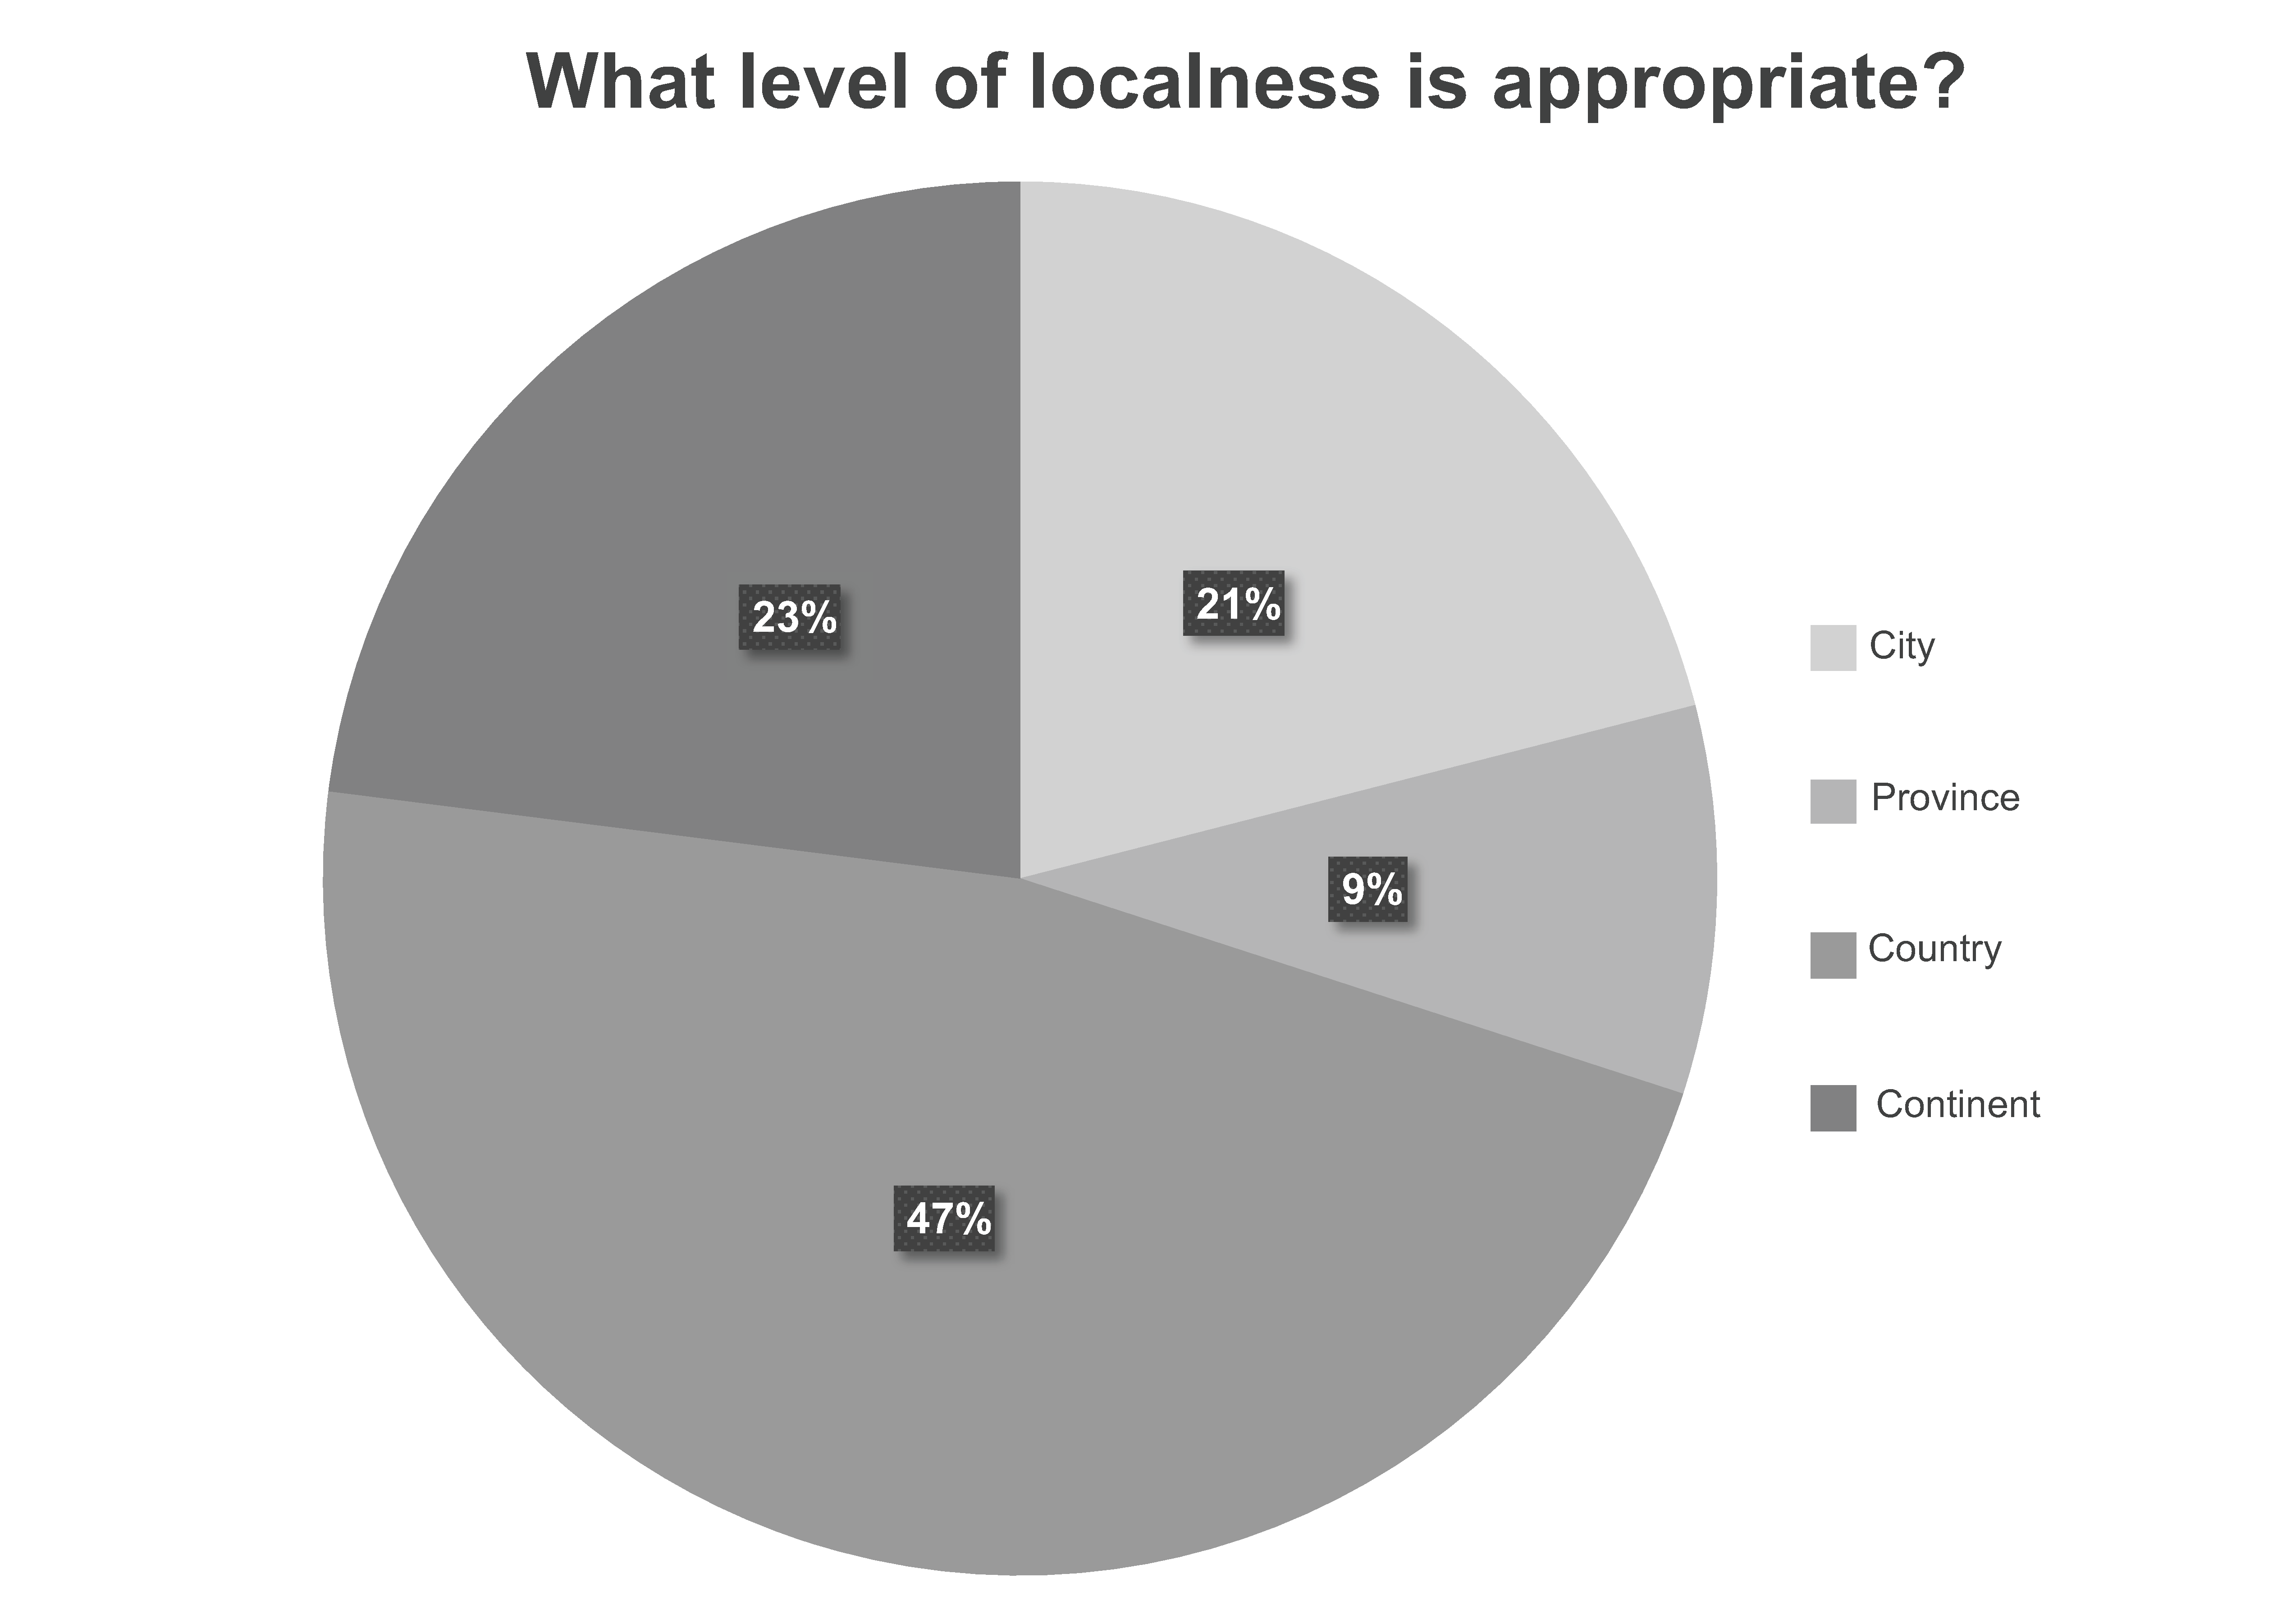
\includegraphics[width=.8\textwidth]{ART_Soloducha/illustration1.pdf}%
 \end{center}%
 \caption{Most interesting results of the survey in terms of clustering of preferences of AV users. Source: Author's study.}\label{sol-ill1}
\end{figure}
%Illustration 1

The responses are split almost equally between the preferences of the driver and the preferences of the residents of the area in which the vehicle travels, with a~slight advantage to the driver. The conclusion for manufacturers of autonomous devices is therefore that a~device should have an open architecture that allows it to be adapted to the preferred option, unless legal regulations decide otherwise. However, as the survey results show, imposing solutions in this area may end in reduced trust in the device.
\begin{figure}
 \begin{center}
 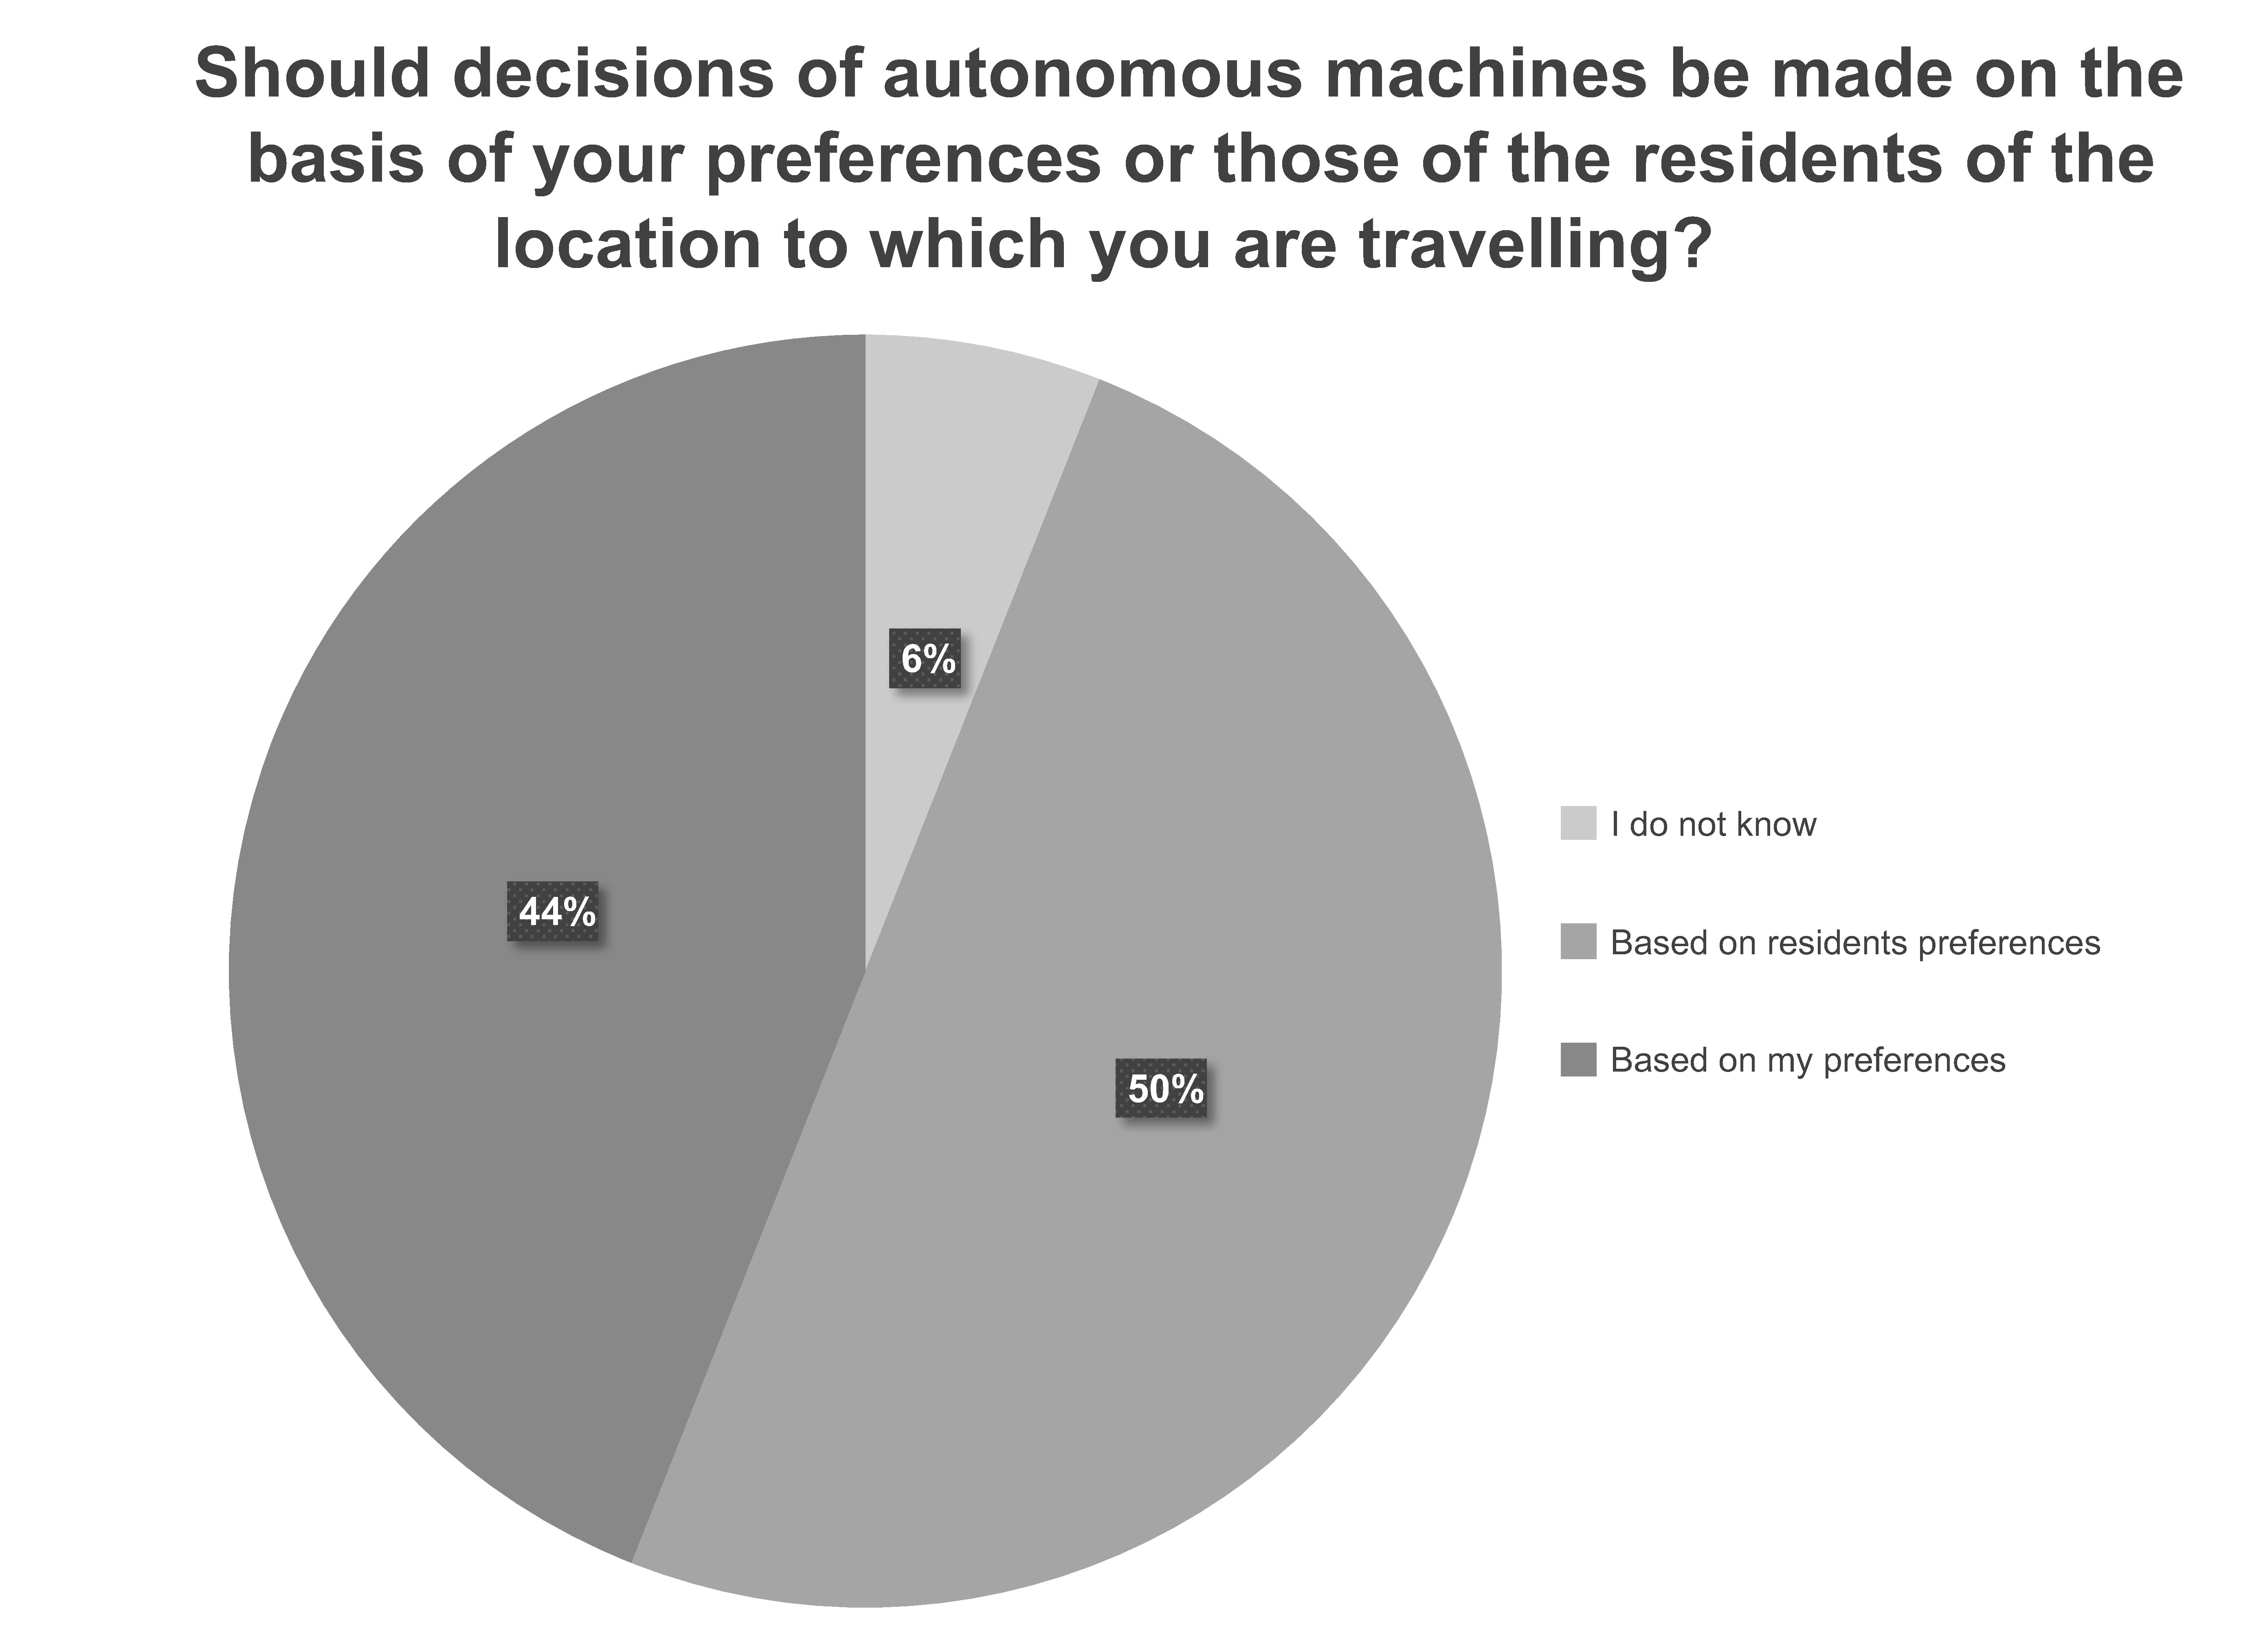
\includegraphics[width=.8\textwidth]{ART_Soloducha/illustration2.pdf}%
 \end{center}%
 \caption{Level of clustering survey. Source: Author's study.}\label{sol-ill2}
\end{figure}
%Illustration 2
%Source: Author's study

The other problem investigated in the survey was the level of clustering. The top level used in the research was the continental one. The majority of respondents preferred the level of state. The level of clustering reflecting Ingelhart-Welzel's map of cultural influences used in the research mentioned above did not appear among the questions. This does not reflect traditional geographical and administrative distinctions.

\section*{Conclusion}
Despite the sceptical voices raised against the practical implementation of the idea of an extrapolated, coherent volition of humanity in the form of the Moral Machine project, it does not seem that this criticism undermines certain important arguments that stand behind Yudkowsky's CEV project and its implementation attempts. In conclusion, we would like to point them out and outline some possible paths for further consideration of this issue.

Firstly, Yudkowsky's project and attempts to implement it are answers to the question of what moral patterns should be introduced into the decision-making procedures of machines so that they meet Giddens' active trust requirements. Any attempts to do this in a~top-down model by enlightened bodies, special committees or top-down adopted normative systems does not meet the criterion of persuasive trust proposed by Giddens. Therefore, the attempt to do this in a~descriptive way through empirical research referring to extrapolation of results of the survey seems a~method tailored to these needs, with all of the doubts associated with the naturalisation of morality and the limitations of descriptive research related to Hume's guillotine problem. Although, in our paper, we tried to show that the weak rationality associated with the inductive approach applied to moral problems can be used to overcome the is-ought problem in the case of the ethics of autonomous machines.

Secondly, such considerations can be conducted under the assumption that the best path to their implementation is to define cognitive processes (including those of a~moral nature) as consisting of information processing. What may help here may be the assumption that such a~definition of moral cognition would not be a~naturalisation
%\label{ref:RNDAVNr8uUo2k}(Rosenbloom, 2015).
\parencite[][]{peruzzi_beginners_2015}. %
 This also could help to eliminate the troubling issue of the \textit{is-ought problem}. Although it is an issue considered by some theorists to be an illusory 
%\label{ref:RNDke81GSJMB7}(Gellner, 2005)
\parencite[][]{gellner_words_2005} %
 and an argument that is treated as untenable nowadays 
%\label{ref:RNDv1WxbP4FgK}(Searle, 1964)
\parencite[][]{searle_how_1964} %
 from point of view of ``weak'' rationality—as mentioned above.

Thirdly, the acceptance of the possibility of clustering moral patterns can lead to the idea of constructing the architecture of autonomous machines as open for adaptation of the patterns used for decision-making to the local characteristics of the user/social environment. The sample survey presented at the end of the paper demonstrates the preferences of a~limited group of respondents regarding this issue.

Fourthly, there is quite advanced research on the technology of so-called social robots, whose task is to produce a~personalised interactive communication experience by considering the preferences of the user the robot interacts with
%\label{ref:RNDaTAZLD4Bt6}(Maroto-Gómez et al., 2022).
\parencite[][]{maroto-gomez_adaptive_2022}. %
 It is based on technology so called preference learning 
%\label{ref:RNDU0HNfJ31Dd}(Fürnkranz and Hüllermeier, 2011).
\parencite[][]{furnkranz_preference_2011}. %
 Using an online survey, participants provide their defining features and preferences towards the activities of the robot. Then, a~preference learning model estimates the preferences of new users using similar features of the survey participants. The survey contains questions about sociodemographic, habits, interests, and preferences about specific attributes related to social robot 
%\label{ref:RNDy6uoBMKwmA}(Fürnkranz and Hüllermeier, 2011, p.2).
\parencite[][p.2]{furnkranz_preference_2011}.%


\paragraph{Acknowledgments.}
The author wishes to thank anonymous helpful referees whose insightful comments helped improve the quality of the present paper. Most certainly, if there are still some errors remaining, they are my own responsibility.



\end{artengenv}

%\section*{References}
%Arrow, K.J., 1973. Some Ordinalist-Utilitarian Notes on Rawls's Theory of Justice. \textit{The Journal of Philosophy}, [online] 70(9), pp.245–263. https://doi.org/10.2307/2025006.
%
%Asimov, I., 2004. Runaround. In: \textit{I, robot}, Bantam spectra book, Bantam hardcover edition. New York: Bantam Books. pp.30–55.
%
%Awad, E., Dsouza, S., Shariff, A., Rahwan, I. and Bonnefon, J.-F., 2020. Universals and variations in moral decisions made in 42 countries by 70,000 participants. \textit{Proceedings of the National Academy of Sciences}, [online] 117(5), pp.2332–2337. https://doi.org/10.1073/pnas.1911517117.
%
%Bigman, Y.E. and Gray, K., 2020. Life and death decisions of autonomous vehicles. \textit{Nature}, [online] 579(7797), pp.E1–E2. https://doi.org/10.1038/s41586-020-1987-4.
%
%Bostrom, N., 2016. \textit{Superintelligence: Paths, Dangers, Strategies}. Oxford: Oxford University Press.
%
%Burrell, J., 2016. How the machine ‘thinks': Understanding opacity in machine learning algorithms. \textit{Big Data \& Society}, [online] 3(1), pp.1–12. https://doi.org/10.1177/2053951715622512.
%
%Czyżowska, D., Niemczyński, A. and Kmieć, E., 1993. Formy rozumowania moralnego Polaków w~świetle danych z~badania metodą Lawrence'a Kohlberga. \textit{Kwartalnik Polskiej Psychologii Rozwojowej}, 2(1), pp.19–38.
%
%Dignum, V., 2022. \textit{Responsible Ai: From Principles to Action}. [online] Michigan Institute for Data Science. Available at: {\textless}https://www.youtube.com/watch?v=LwKDOwwJpL4{\textgreater} [Accessed 11 January 2023].
%
%Edmonds, E., 2017. \textit{Americans Feel Unsafe Sharing the Road with Fully Self-Driving Cars}. [online] AAA Newsroom. Available at: {\textless}https://newsroom.aaa.com/2017/03/americans-feel-unsafe-sharing-road-fully-self-driving-cars/{\textgreater} [Accessed 11 January 2023].
%
%Eschenbach, W.J. von, 2021. Transparency and the Black Box Problem: Why We Do Not Trust AI. \textit{Philosophy \& Technology}, [online] 34(4), pp.1607–1622. https://doi.org/10.1007/s13347-021-00477-0.
%
%Foot, P., 2002. \textit{Virtues and Vices}. [online] Oxford University Press. https://doi.org/10.1093/0199252866.001.0001.
%
%Fukuyama, F., 1995. \textit{Trust: the social virtues and the creation of prosperity}. 1st ed. A~Free Press paperbacks book. New York: Free Press.
%
%Fürnkranz, J. and Hüllermeier, E., 2011. Preference Learning: An Introduction. In: J. Fürnkranz and E. Hüllermeier, eds. \textit{Preference Learning}. [online] Berlin, Heidelberg: Springer. pp.1–17. https://doi.org/10.1007/978-3-642-14125-6\_1.
%
%Gellner, E., 2005. \textit{Words and Things: An Examination of, and an Attack on, Linguistic Philosophy}. 1. publ ed. Routledge classics. London: Routledge.
%
%Giddens, A., 1991. \textit{Modernity and Self-Identity: Self and Society in the Late Modern Age}. Stanford, CA: Stanford University Press.
%
%Górnicka, J., 1980. Rozwój moralny w~koncepcji Lawrence'a Kohlberga. \textit{Człowiek i~Światopogląd}, 6, pp.113–123.
%
%Greene, J.D., 2013. \textit{Moral Tribes: Emotion, Reason, and the Gap Between Us and Them}. London: Atlantic Books.
%
%Gryz, J., 2021. \textit{Sztuczna~Inteligencja:~powstanie,~rozwój,~rokowania}. [online] Copernicus Center. Available at: {\textless}https://www.youtube.com/watch?v=3ZDfVgC897k{\textgreater} [Accessed 11 January 2023].
%
%Harsanyi, J.C., 1975. Can the Maximin Principle Serve as a~Basis for Morality? A~Critique of John Rawls's Theory. \textit{The American Political Science Review}, [online] 69(2), pp.594–606. https://doi.org/10.2307/1959090.
%
%Hofstede, G.H., Hofstede, G.J. and Minkov, M., 2010. \textit{Cultures and Organizations: Software of the Mind: Intercultural Cooperation and Its Importance for Survival}. 3rd ed ed. New York: McGraw-Hill.
%
%Hofstede, G.J., 2011. \textit{Geert Hofstede on Culture}. [online] Viewdutch. Available at: {\textless}https://www.youtube.com/watch?v=wdh40kgyYOY{\textgreater} [Accessed 11 January 2023].
%
%Holstein, T. and Dodig-Crnkovic, G., 2018. Avoiding the intrinsic unfairness of the trolley problem. In: \textit{Proceedings of the International Workshop on Software Fairness}. [online] ICSE '18: 40th International Conference on Software Engineering. Gothenburg Sweden: ACM. pp.32–37. https://doi.org/10.1145/3194770.3194772.
%
%Inglehart, R. and Welzel, C., 2005. \textit{Modernization, Cultural Change, and Democracy: The Human Development Sequence}. [online] Cambridge: Cambridge University Press. https://doi.org/10.1017/CBO9780511790881.
%
%Jörgensen, J., 1937. Imperatives and logic. \textit{Erkenntnis}, [online] 7(1), pp.288–296. https://doi.org/10.1007/BF00666538.
%
%Karpus, J., Krüger, A., Verba, J.T., Bahrami, B. and Deroy, O., 2021. Algorithm exploitation: Humans are keen to exploit benevolent AI. \textit{iScience}, [online] 24(6), p.102679. https://doi.org/10.1016/j.isci.2021.102679.
%
%Kohlberg, L., 1958. \textit{The Development of Modes of Moral Thinking and Choice in the Years 10 to 16}. [PhD thesis] University of Chicago. Available at: {\textless}https://www.proquest.com/openview/c503bf59d762abe5818e1b24c484d41a/1?pq-origsite=gscholar\&cbl=18750\&diss=y{\textgreater} [Accessed 11 January 2023].
%
%Lo, T., 2019. \textit{My Amazon Alexa Went Rogue and Ordered Me to Stab Myself in the Heart}. [online] Mirror Online. Available at: {\textless}https://www.mirror.co.uk/news/uk-news/my-amazon-echo-went-rogue-21127994{\textgreater} [Accessed 11 January 2023].
%
%Maroto-Gómez, M., Castro-González, Á., Castillo, J.C., Malfaz, M. and Salichs, M.Á., 2022. An adaptive decision-making system supported on user preference predictions for human–robot interactive communication. \textit{User Modeling and User-Adapted Interaction}, [online] pp.1–45. https://doi.org/10.1007/s11257-022-09321-2.
%
%Miłaszewicz, D., 2016. Zaufanie jako wartość społeczna. \textit{Studia Ekonomiczne}, [online] (259), pp.80–88. Available at: {\textless}http://cejsh.icm.edu.pl/cejsh/element/bwmeta1.element.cejsh-d64b921a-5db7-4208-9eb7-73baaa05f7e4{\textgreater} [Accessed 11 January 2023].
%
%Mirnig, A.G. and Meschtscherjakov, A., 2019. Trolled by the Trolley Problem: On What Matters for Ethical Decision Making in Automated Vehicles. In: \textit{Proceedings of the 2019 CHI Conference on Human Factors in Computing Systems}. [online] CHI '19: CHI Conference on Human Factors in Computing Systems. Glasgow Scotland Uk: ACM. pp.1–10. https://doi.org/10.1145/3290605.3300739.
%
%Nagel, T., 1986. \textit{The View from Nowhere}. 1st ed. Oxford: Oxford University Press.
%
%Nozick, R., 2013. \textit{Anarchy, State, and Utopia}. New York: Basic Books.
%
%Pasquale, F., 2016. \textit{The Black Box Society: The Secret Algorithms That Control Money and Information}. Cambridge, MA: Harvard University Press.
%
%Rawls, J., 1971. \textit{A~Theory of Justice}. [online] Cambridge, MA: The Belknap Press of Harvard University Press. Available at: {\textless}http://www.gbv.de/dms/bowker/toc/9780674880146.pdf{\textgreater} [Accessed 11 January 2023].
%
%Rosenbloom, P., 2015. \textit{On Computing: The Fourth Great Scientific Domain}. Cambridge, MA: The MIT Press.
%
%Searle, J.R., 1964. How to Derive ‘Ought' From ‘Is'. \textit{The Philosophical Review}, [online] 73(1), pp.43–58. https://doi.org/10.2307/2183201.
%
%Wysocki, I., 2021. The problem of indifference and homogeneity in Austrian economics: Nozick's challenge revisited. \textit{Philosophical Problems in Science (Zagadnienia Filozoficzne w~Nauce}), [online] (71), pp.9–44. Available at: {\textless}https://zfn.edu.pl/index.php/zfn/article/view/554{\textgreater} [Accessed 24 January 2022].
%
%Yudkowsky, E., 2004. \textit{Coherent Extrapolated Volition}. San Francisco, CA: San Francisco.
%\end{document}
